\section{Backpressure}\label{sec:backpressure}

\begin{frame}{{\nameref{sec:backpressure}}}
    \centering
    \Large
    Hot vs Cold Observables
\end{frame}

\begin{frame}{{\nameref{sec:backpressure}}}
    \begin{itemize}
    	\item \textbf{Cold}: Emit on subscribe(), starting from the beginning
    	\item \textbf{Hot}: Emit constantly, subscribers \enquote{tune} in and out
    \end{itemize}
\end{frame}

\begin{frame}{Backpressure Strategies}
	\begin{itemize}
		\item \textbf{Error}: Signals a MissingBackpressureException. %deadend
        \begin{figure}[h]
			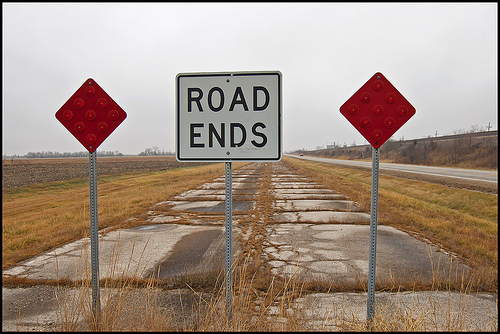
\includegraphics[width=0.8\textwidth,page=1]{gfx/roadend.jpg}
		\end{figure}
    \end{itemize}
\end{frame}

\begin{frame}{Backpressure Strategies}
	\begin{itemize}
    	\item \textbf{Buffer}: Buffers all onNext values. %dam
        \begin{figure}[h]
			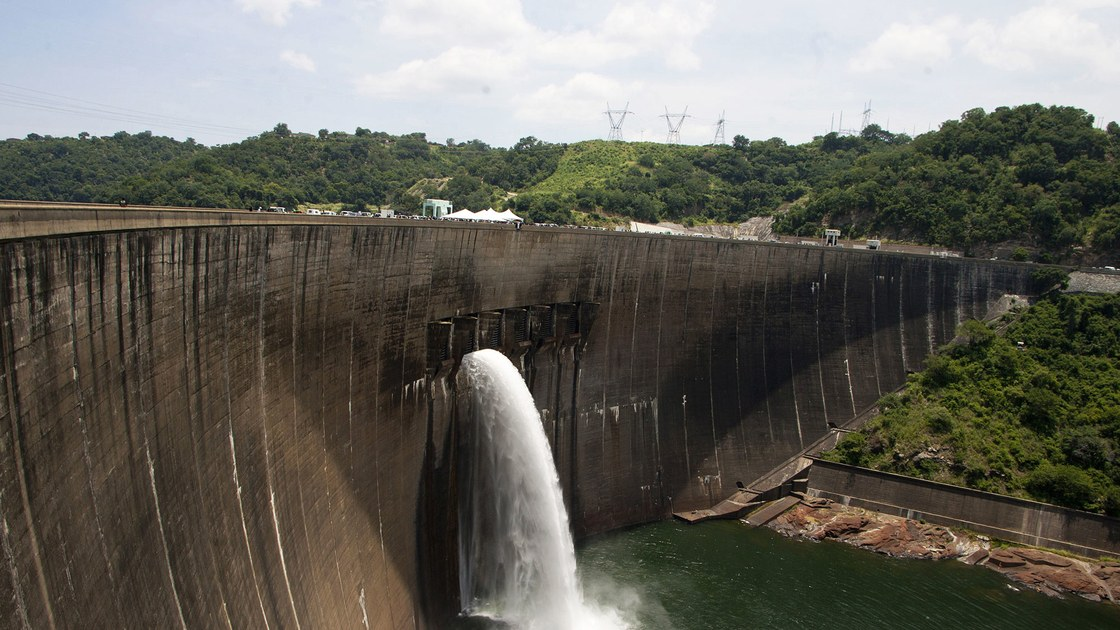
\includegraphics[width=0.9\textwidth,page=1]{gfx/dam.jpg}
		\end{figure}
	\end{itemize}
\end{frame}

\begin{frame}{Backpressure Strategies}
	\begin{itemize}
    	\item \textbf{Drop}: Drops the most recent onNext value. %overflow
        \begin{figure}[h]
			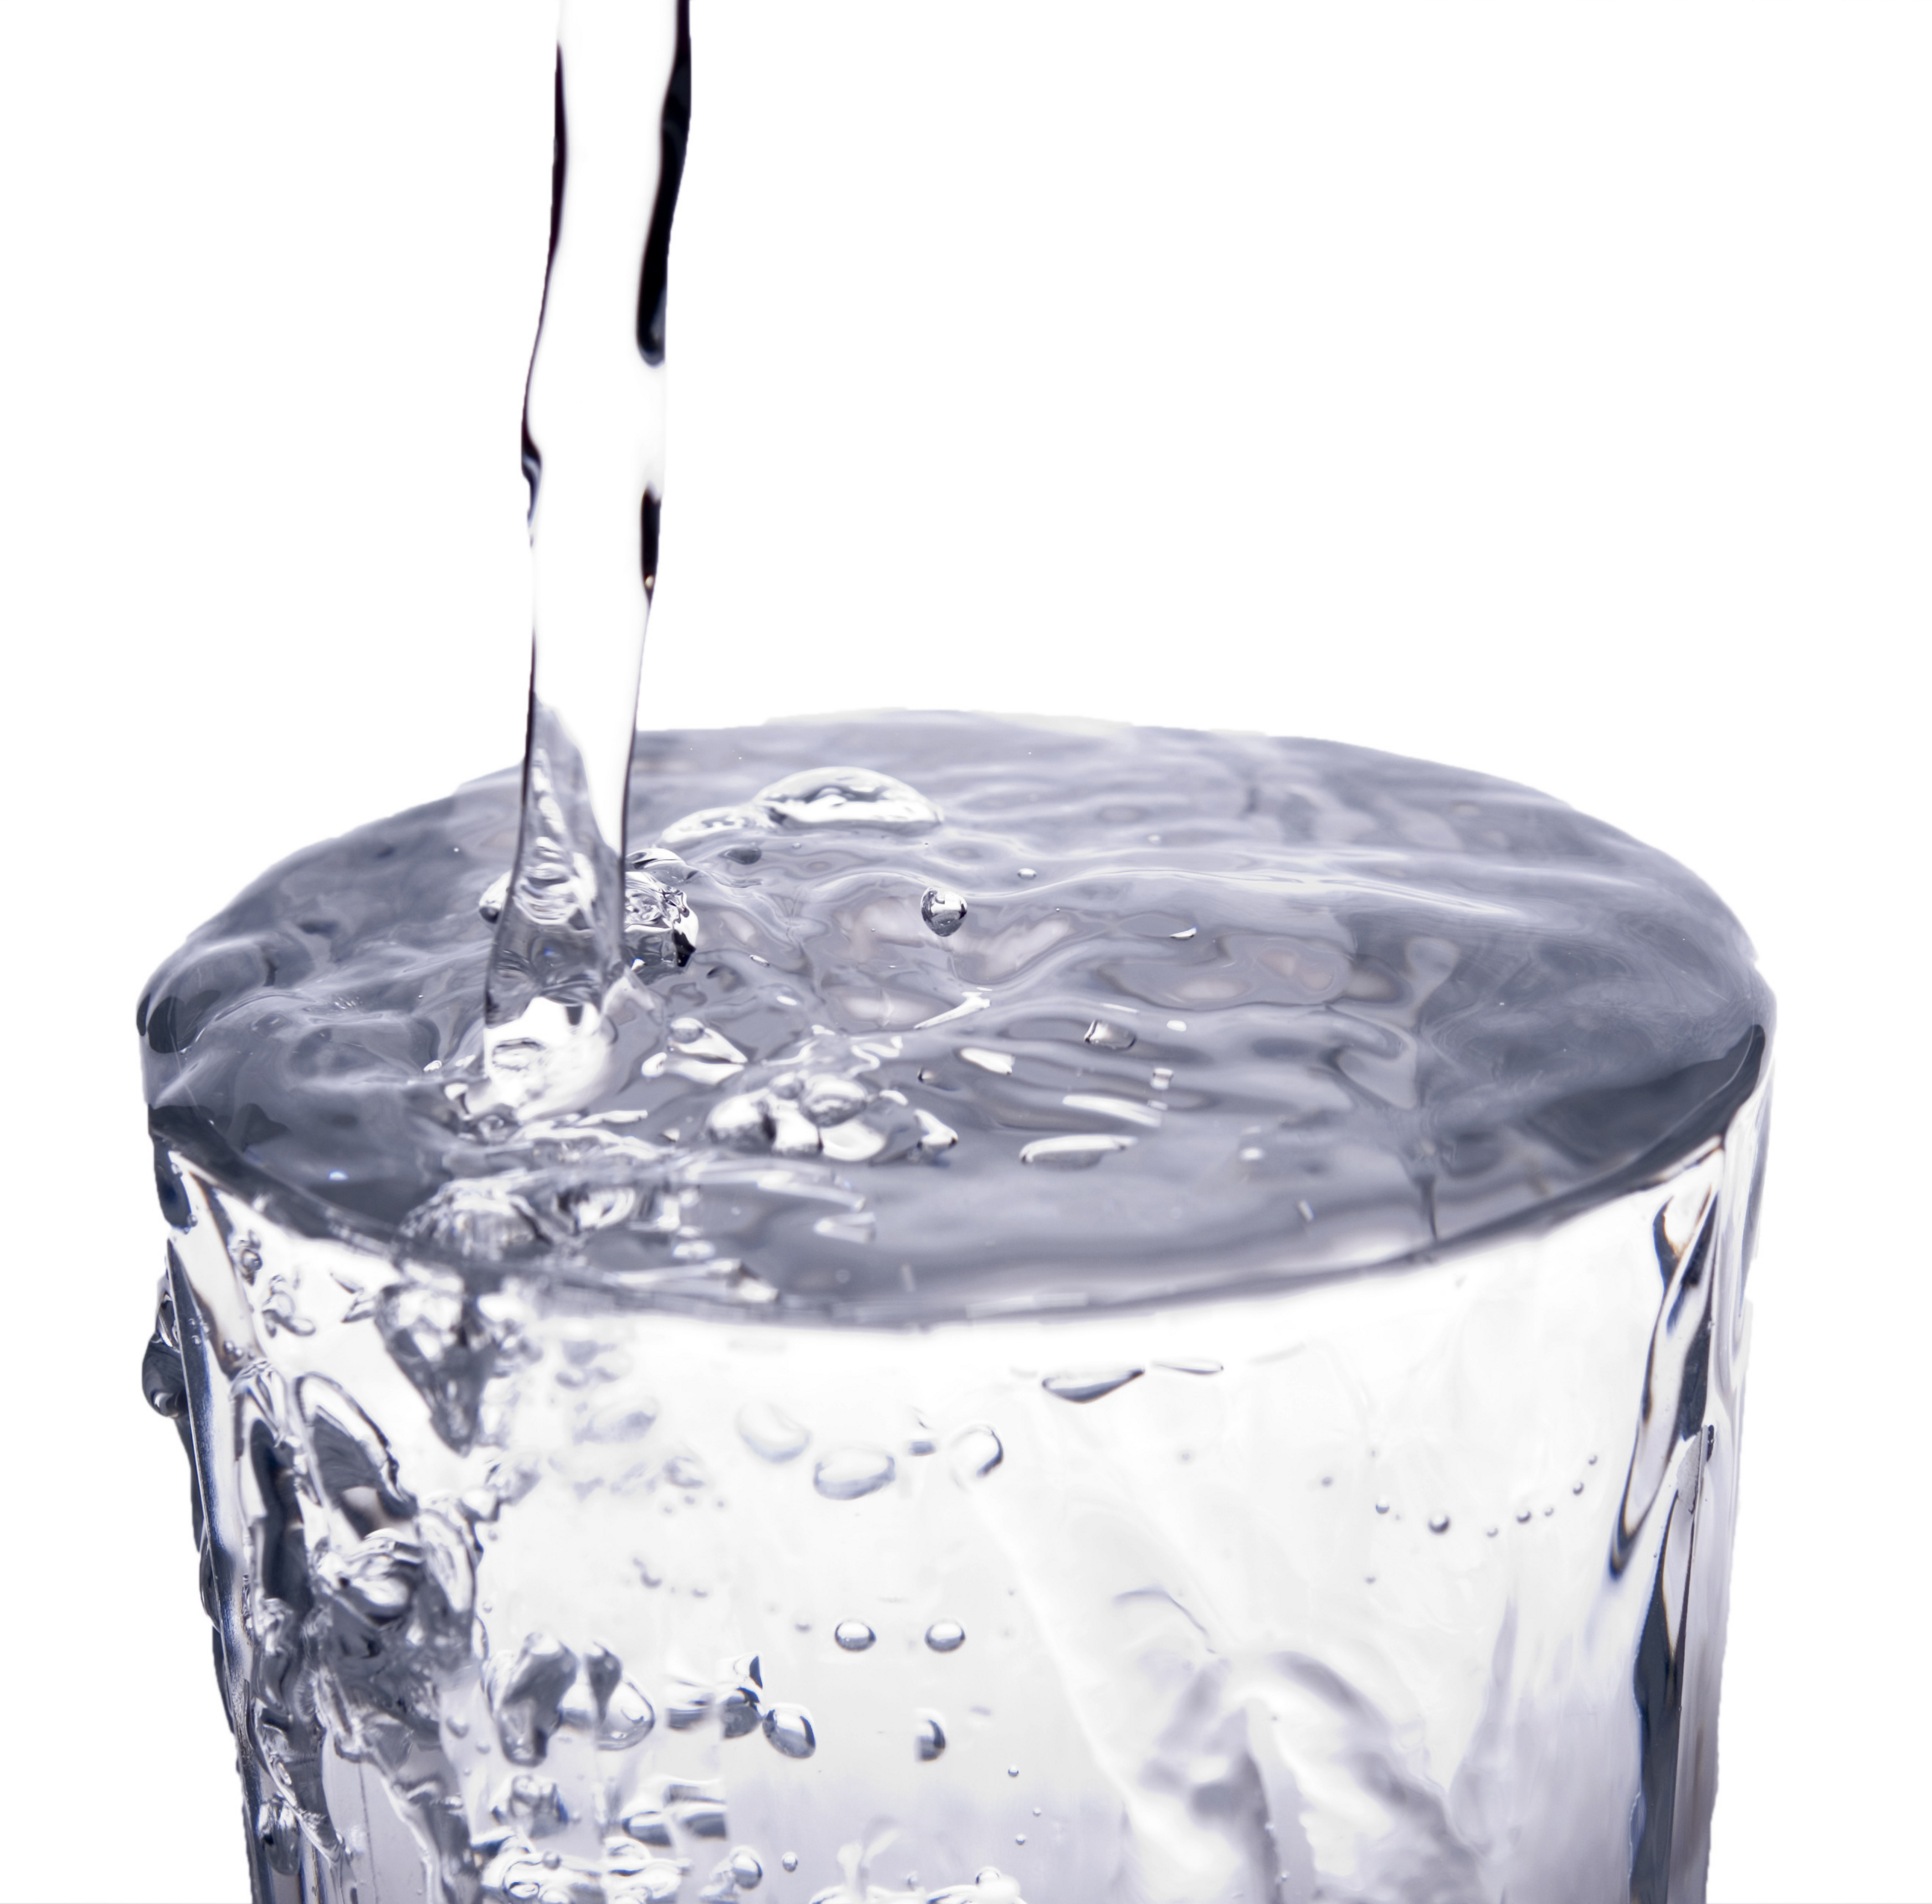
\includegraphics[width=0.6\textwidth,page=1]{gfx/Overflow.jpg}
		\end{figure}
	\end{itemize}
\end{frame}

\begin{frame}{Backpressure Strategies}
	\begin{itemize}
        \item \textbf{Latest}: Keeps only the latest onNext value, overwriting any previous value. %highway exit sign
        \begin{figure}[h]
			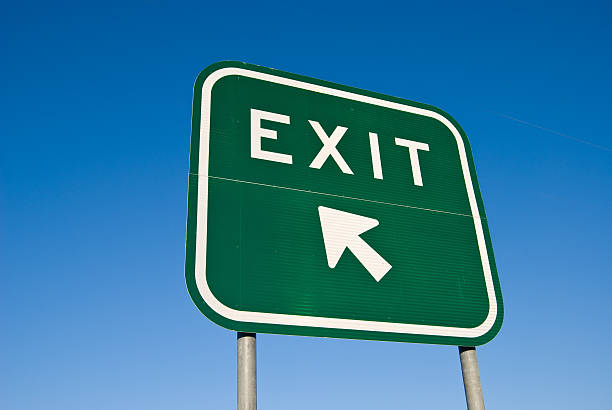
\includegraphics[width=0.8\textwidth,page=1]{gfx/exit.jpg}
		\end{figure}
	\end{itemize}
\end{frame}

\begin{frame}{Backpressure Strategies}
	\begin{itemize}
        \item \textbf{Missing}: OnNext events are written without any buffering or dropping. %no strategy
            \begin{figure}[h]
			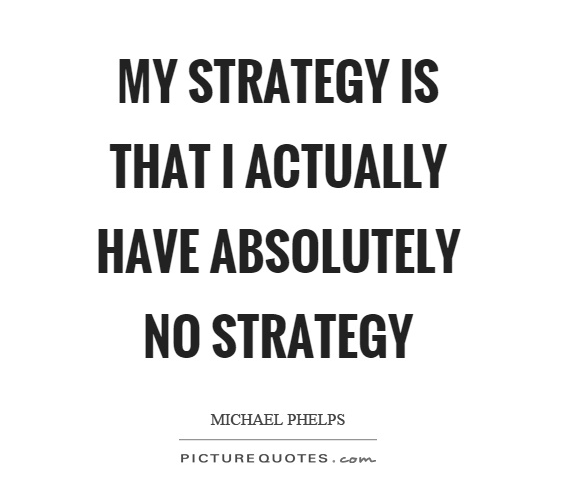
\includegraphics[width=0.7\textwidth,page=1]{gfx/NoStrategy}
		\end{figure}
	\end{itemize}
\end{frame}

%     Backpressure Strategies\\
%     managing hot observables (debounce, sample etc)
